
%%%%%%%%%%%%%%%%%%%%%%%%%%%%%%%%%%%%%%%%%%%
%%%%%%  STYLE 02
%%%%%%%%%%%%%%%%%%%%%%%%%%%%%%%%%%%%%%%%%%%
\clearpage

\cxset{
 name={},
 numbering=arabic,
 number font-size=\LARGE,
 number font-family=\rmfamily,
 number font-weight=\bfseries,
 number before=,
 number dot=.,
 number after=\hspace{1em},
 number position=rightname,
 chapter font-family=\sffamily,
 chapter font-weight=\normalfont,
 chapter font-size=\Large,
 chapter before={\vspace*{20pt}\par\hfill},
 chapter after={},
 chapter color={black!90},
 number color=thered,
 title beforeskip={},
 title afterskip={\vspace*{50pt}\par},
 title before={},
 title after={},
 title font-family=\sffamily,
 title font-color= thered,
 title font-weight=\bfseries,
 title font-size=\LARGE}

\chapter{Style 2}
\parindent0pt
I tend to favour this design for books that have a lot of pictures. It brings the design into the margins and leaves plentiful white space in the margins. From a programming point of view the chapter is the opposite of openany. It has to open on an odd number.
\medskip
\begin{figure}[ht]
\centering
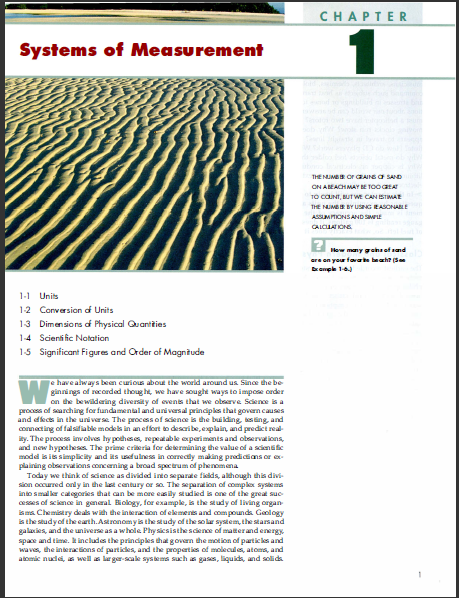
\includegraphics[width=0.6\textwidth]{./chapters/chapter02}
\end{figure}

